
\subsection{Ease of use}
As described by \citet{easeOfUse}, the perceived ease of use is "the degree to which a person believes that using a particular system would be free of effort". In terms of the technology and argumentation framework solvers, this can be translated to the effort required to setup those systems, and the learning curve on how to use them. 

In terms of the usage of the solvers submitted to ICCMA 2017 competition, they are all developed as a autonomous systems with command line interface. Due to the requirements of the competition, they all implement the same command line arguments:

\begin{itemize}
	\item -f \textless file\textgreater - specifies the path to the file with argumentation framework
	\item -p \textless task\textgreater - specifies the tasks that should be performed
	\item -fo \textless fileformat\textgreater - specifies the format of the file for argumentation framework: apx or tgf
\end{itemize}

Majority of ICCMA 2017 solvers are implemented in C++ programming language, with few exception like goDiamond \citep{goDiamond}, which is implemented using Go language \citep{GoLang}, or Pyglaf \citep{pyglaf}, where is a mix of Python and C++ programming languages. 



\subsubsection{Setup And Installation}
Throughout the project, there was an attempt to setup four systems from ICCMA 2017 on the testing machine: Pyglaf \citep{pyglaf}, ArgSem-SAT \citep{argsemsat}, ArgTools \citep{argtools} and argmat-clpb \citep{argmat-clpb}. 

\paragraph{Pyglaf}
As seen in section \ref{section:pyglaf}, Pyglaf is implemented using Python for building encodings of semantics and C++ programming language for the main solver. Hence, in order to use Pyglaf, user has to manually build Circumscriptino \citep{circumscriptino} solver and either provide the path to it to Pyglaf, or move it to the same folder as Pyglaf executable exists. The source code for pyglaf and Circumsriptino can be obtained either from GitHub or all required files compressed together can be found on Mark Alviano website \textit{https://alviano.com/software/pyglaf/}. Although, Pyglaf won the most track in ICCMA 2017 competition, the steps required to set it up can be troublesome, especially for someone with limited technological skills. 

\paragraph{ArgSem-SAT}
Similarly to Pyglaf, in order to use ArgSem-SAT solver, user is required to build the source code himself. However, ArgSem-SAT source code is not easily available through any version control systems, but instead can be found on Source Forge website \textit{https://sourceforge.net/projects/argsemsat/}. The build script is provided together with the source code, which helps with the set up of the solver. However, ArgSem-SAT is dependent on the STLSoft C++ library \citep{stlsoft}, which is providing facades over operating-system and technology specific APIs and Standard Template Library. The problem starts when user tries to build solver using any latest version of the GCC Compiler \citep{gcc}. As shown in figure \ref{fig:argsemsatBuildError}, the STLSoft library only supports GCC compilers up to version 4. However, the latest released version of GCC is 8.2 as of July 2018 \citep{gcc} and any up to date Linux distribution will use version 5 or higher. Hence, in order to use ArgSem-SAT the user is forced to downgrade the compiler. Although this resolved the issues with setting up ArgSem-SAT, this again can be troublesome and problematic for certain users.

\begin{figure}[h]
	\centering
	\includegraphics[width=\linewidth]{"img/argsemsat_error"}
	\caption{ArgSem-SAT build error}
	\label{fig:argsemsatBuildError}
\end{figure}

\paragraph{argmat-clpb}
Similarly to ArgSem-SAT, argmat-clpb \citep{argmat-clpb} is difficult to setup. Argmat-clpb is part of the larger collection of tools in \textit{argumatrix} project. Based on the documentation available on GitHub page \citep{argmat-clpbGithub}, the project has couple of dependencies: Boos and SWI-Prolog. Although the documentation provides steps required to setup the environment, when user tries to build argmat-clpb, the compiler throws an error as shown in figure \ref{fig:argmatClpbError}. Hence, it was not possible to setup argmat-clpb in the test environment.

\begin{figure}[h]
	\centering
	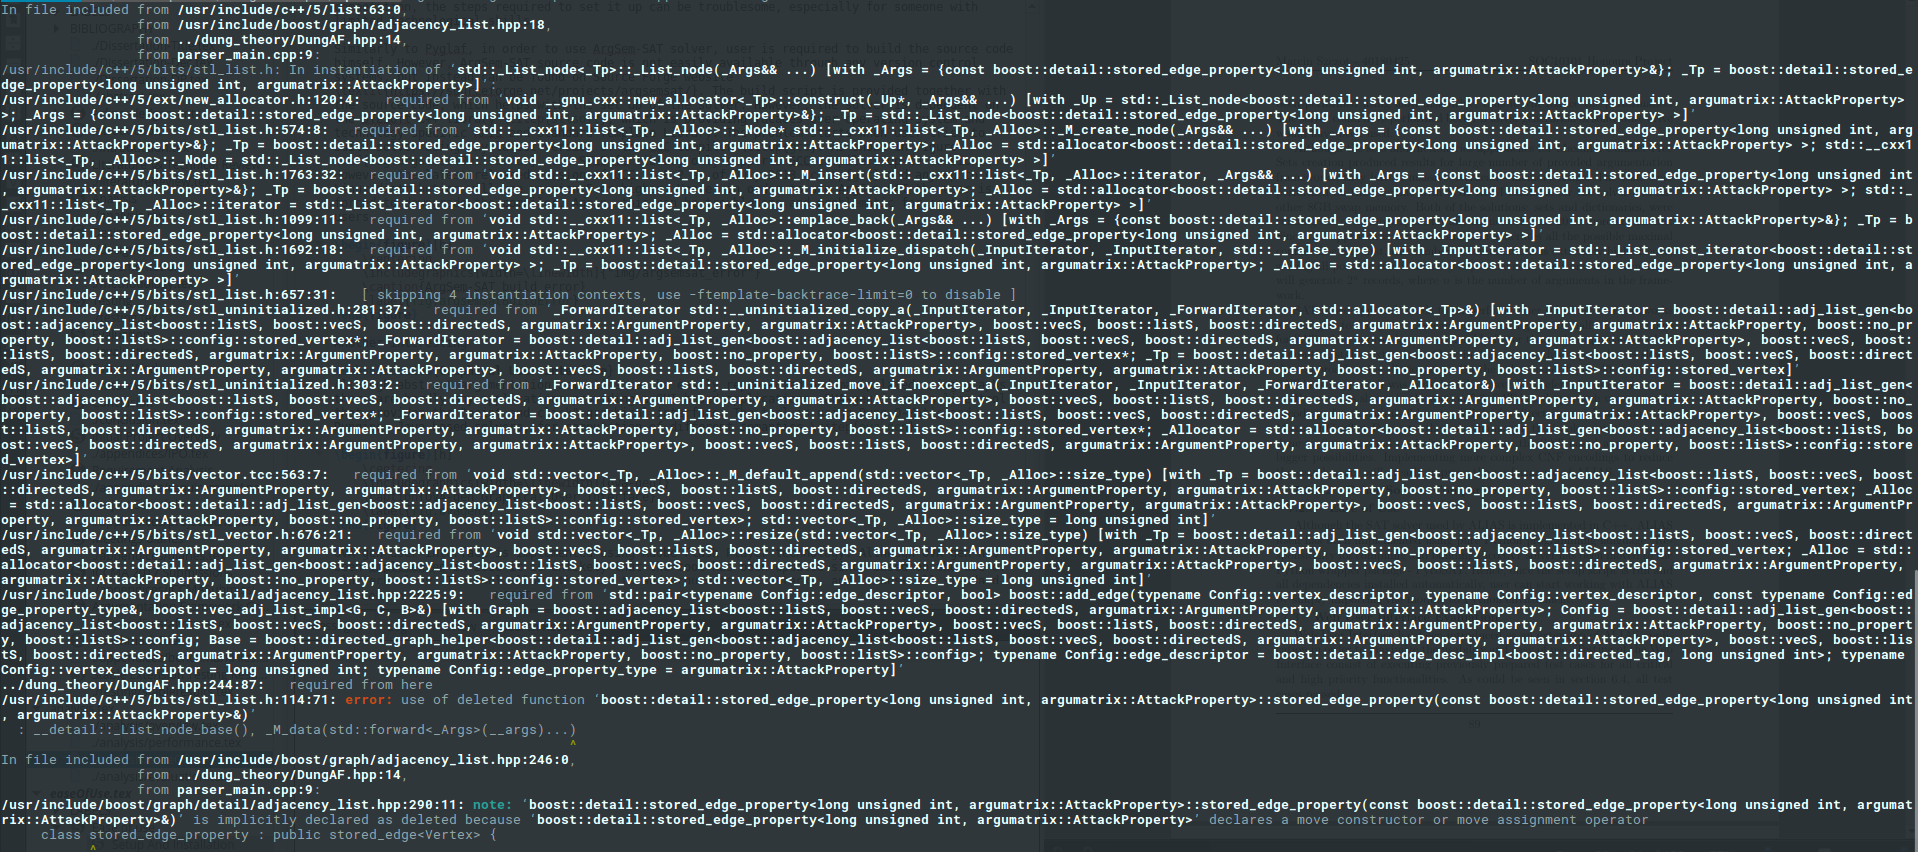
\includegraphics[width=\textwidth]{argmat-clpbError}
	\caption{argmat-clpb build error}
	\label{fig:argmatClpbError}
\end{figure}

\paragraph{ArgTools}
ArgTools, similarly to ArgSem-SAT is not available through any well known source control like GitHub. Instead, solver can be obtained from Source Forge link: \textit{https://sourceforge.net/projects/argtools/}. However, the most recent files for the ArgTools solver contain only number of argumentation frameworks and no source files. Hence, ArgTools solver has not been setup on the test machine.


\subsubsection{Graphical User Interface}
Although abstract argumentation semantics can be easily represented and manipulated using graphs, there are hardly any applications providing a GUI based applications. OVA-gen is an on-line tool that provides the "point and click" graphical interface. The tool is using Dung-O-Matic and Dungine, Java based solvers, for computation of different semantics \citep{ova-gen}. 

\begin{figure}[h]
	\centering
	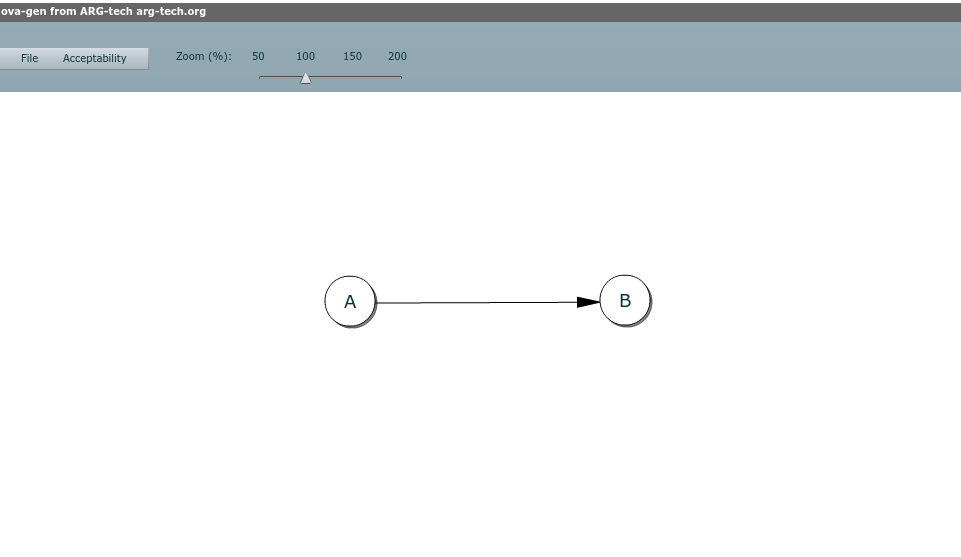
\includegraphics[width=\linewidth]{ova-gen1}
	\caption{OVA-gen Graphical User Interface}
	\label{fig:ovagen1}
\end{figure}

OVA-gen user interface is implemented using Adobe Flash Player technology. Although OVA-gen has been implemented in 2010 it is unlikely that the tool has been updated since based on the use of old technology. The tool allows the user to add arguments and attacks, and request all standard semantics to be computed. Figure \ref{fig:ovagen1} shows the simple argumentation framework representation in OVA-gen.

\begin{figure}[h]
	\centering
	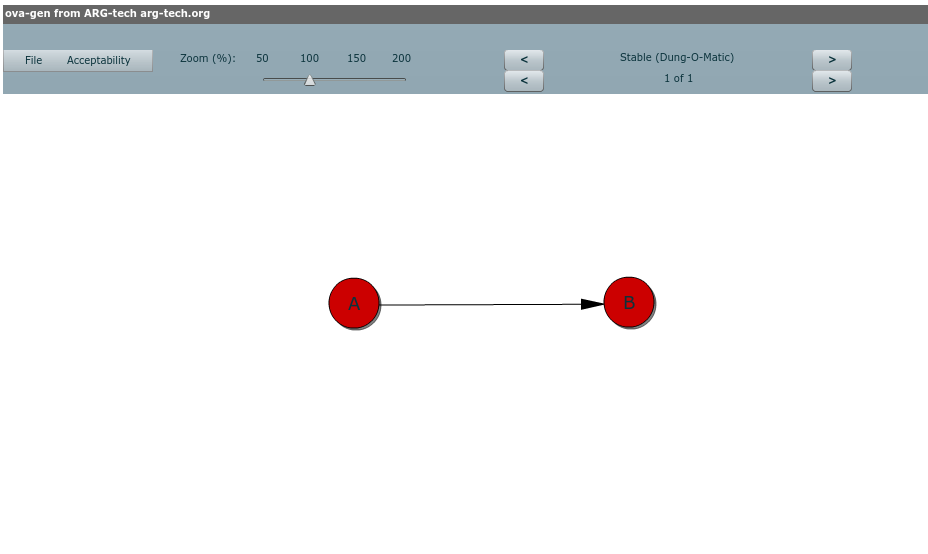
\includegraphics[width=\linewidth]{ova-gen2}
	\caption{OVA-gen Graphical User Interface - Stable Semantic}
	\label{fig:ovagen2}
\end{figure}

One of the problems with OVA-gen is very unclear design. User can only add argument by left-click on the graph area and attack by holding 'Shift' key and clicking two arguments. This is not obvious for the user straight away. The toolbar only offer ability to save and/or clear existing argumentation framework and select the required extension. 

Simple test has been performed with OVA-gen. Argumentation framework has been created with two arguments: $a$ and $b$, and relation $a \implies b$. When any available extension is requested, both arguments are marked with red colour. This would indicate that both arguments are not accepted. However, in this case, argument $a$ should be accepted in majority, if not all of the extensions. Thus, although OVA-gen provides the graphical interface for abstract argumentation frameworks, it does not provide correct results in terms of semantics.